\chapter{Experiments} \label{experiments}
We have carried out three experiments. The goal of the first two experiments was
to test some specific hyperparameter settings of our system. First, we compared
different sampling strategies (section \ref{sec:exp:sample}), then we
experimented with the usage of genetic operators (section \ref{sec:exp:genop}).
The last experiment encompasses runs of our system on the OpenML-CC18 benchmarking
suite.
% TODO cite

\section{Sampling strategies} \label{sec:exp:sample}
In section \ref{sec:scoresample} we presented two different sampling strategies
--- either a sample of the original dataset is generated for every individual
evaluation (\emph{per-ind}), or only once per generation (\emph{per-gen}) and
is shared by all individuals. The goal of this experiment was to test whether
one approach is better.

The strategies were tested on three different datasets:
\begin{itemize}
\item wilt --- Medium size dataset (4839 instances, 6 features), the task is to
detect diseased trees in image segments. There are two target classes: `w' (diseased
trees) and `n' (all other land cover), only few instances of the `w' class
are present (261) \citep{doi:10.1080/01431161.2013.810825}.
\item wine-quality-white --- Medium size dataset (4898 instances, 12 features),
the features represent properties of a particular Portuguese wine. Each of the
wines has been graded by three experts according to sensory properties, the
target value is a median of these grades. The task is to predict the target
grading (1--7), which may be either a classification or a regression task.
\citep{CORTEZ2009547}
\item MagicTelescope --- Large dataset (19020 instances, 12 features), the task
is to determine whether the data produced by the Cherenkov gamma telescope
describes a `signal' or only `background data'. \citep{BOCK2004511}
\end{itemize}

Sample size was chosen proportionally to the dataset size to reduce the running
time --- $\frac{1}{4}$ of all instances in case of the medium-sized datasets
and $\frac{1}{20}$ of the MagicTelescope dataset. The evaluation method
was 10 times 10-fold cross-validation per strategy.

% TODO maybe one pyplot with 3 figures
% TODO check if it still is pdf/a :-) :-) :-)
\begin{figure}[ht]\centering
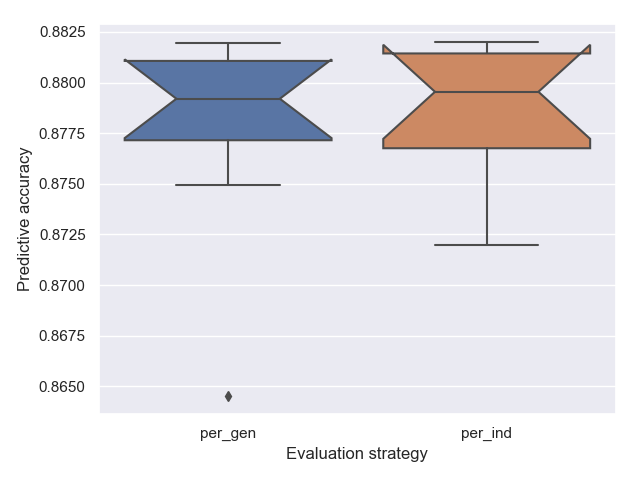
\includegraphics[width=0.7\textwidth]{../img/magic-out.png}
\caption{magic}
\label{pic04:magic}
\end{figure}

\begin{figure}[ht]\centering
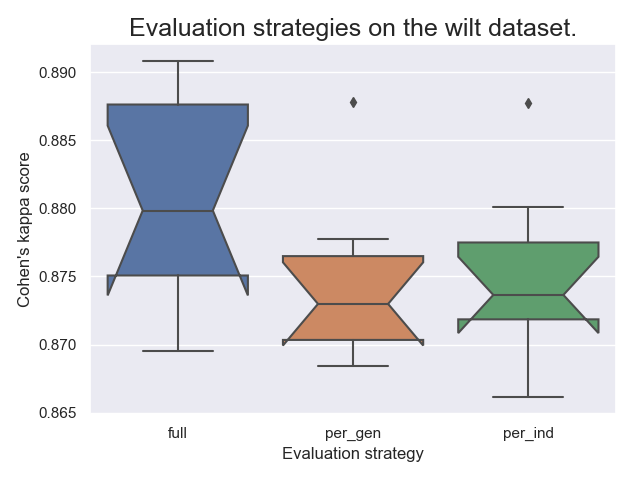
\includegraphics[width=0.7\textwidth]{../img/wilt-out.png}
\caption{wilt}
\label{pic04:wilt}
\end{figure}

\begin{figure}[ht]\centering
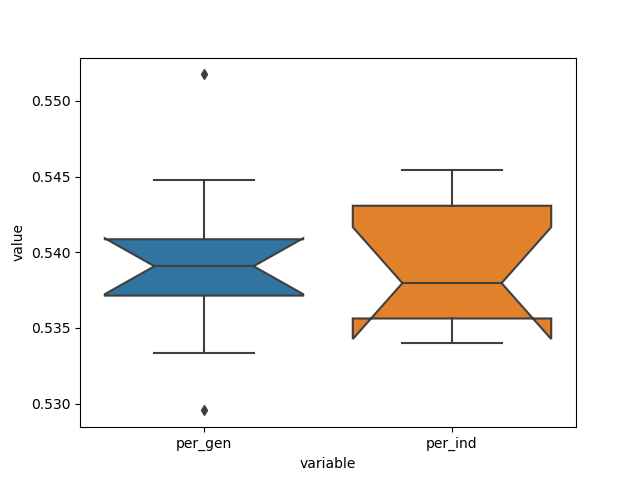
\includegraphics[width=0.7\textwidth]{../img/winequality-out.png}
\caption{wine-quality-white}
\label{pic04:winequality}
\end{figure}

\begin{sidewaysfigure}[ht]
    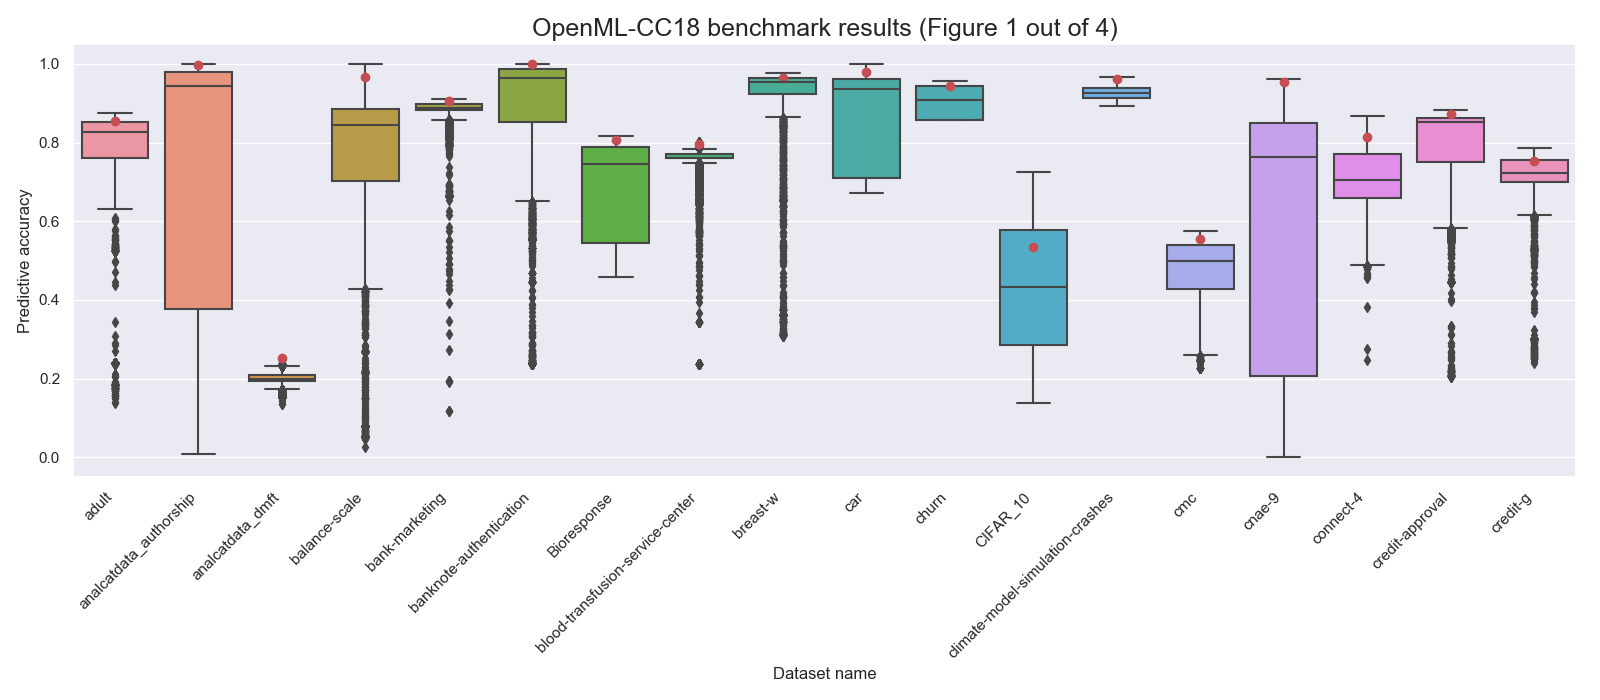
\includegraphics[width=\textwidth]{../img/openml-boxplot0.png}
    \caption[OpenML-CC18 benchmark result comparison (Figure 1 out of 4)]{
    OpenML-CC18 benchmark result comparison (Figure 1 out of 4).
    Boxplots visualize distributions of predictive accuracies of all
    runs uploaded to OpenML.}
    \label{fig:OpenML:boxplot:0}
\end{sidewaysfigure}

\begin{sidewaysfigure}[ht]
    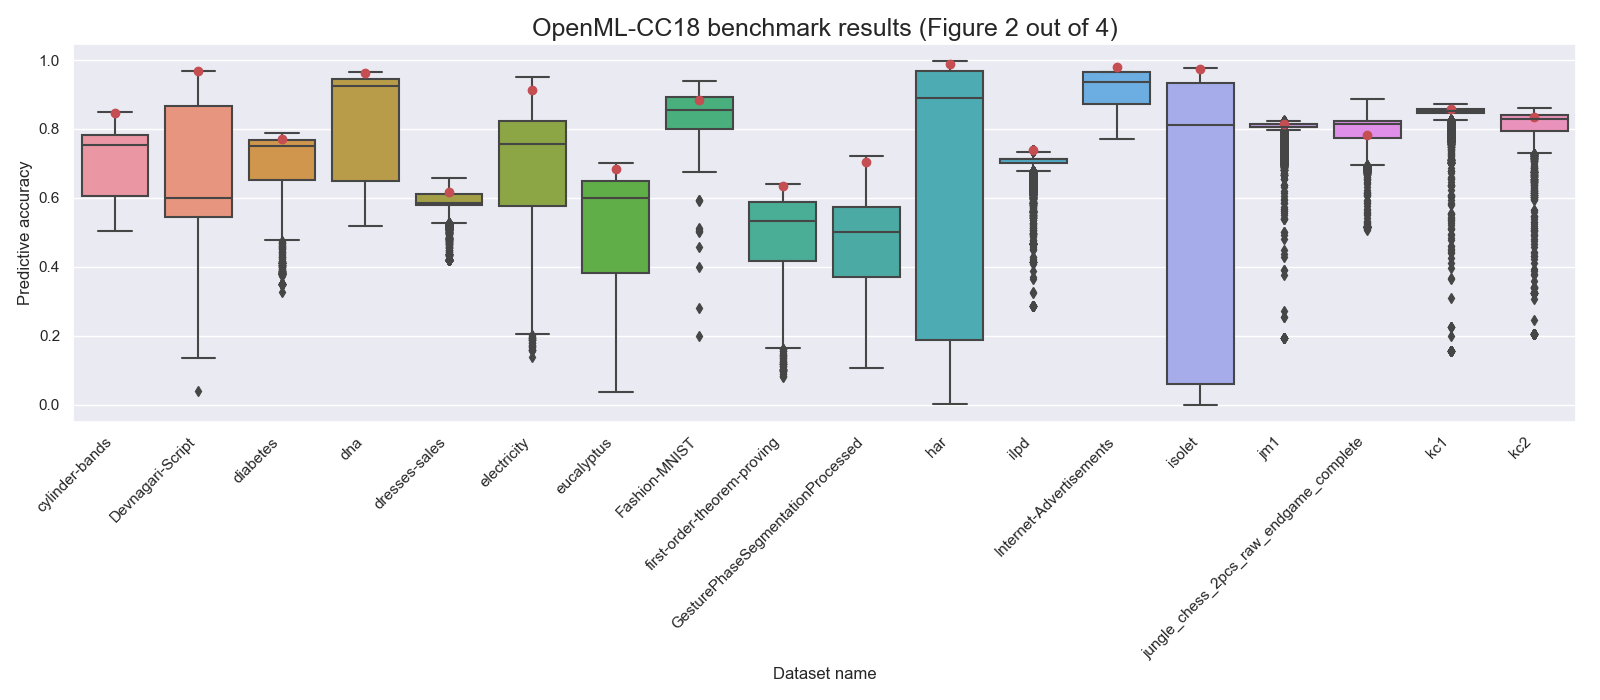
\includegraphics[width=\textwidth]{../img/openml-boxplot1.png}
    \caption[OpenML-CC18 benchmark result comparison (Figure 2 out of 4)]{
	OpenML-CC18 benchmark result comparison (Figure 2 out of 4).    
    Boxplots visualize distributions of predictive accuracies of all
    runs uploaded to OpenML.}
    \label{fig:OpenML:boxplot:1}
\end{sidewaysfigure}

\begin{sidewaysfigure}[ht]
    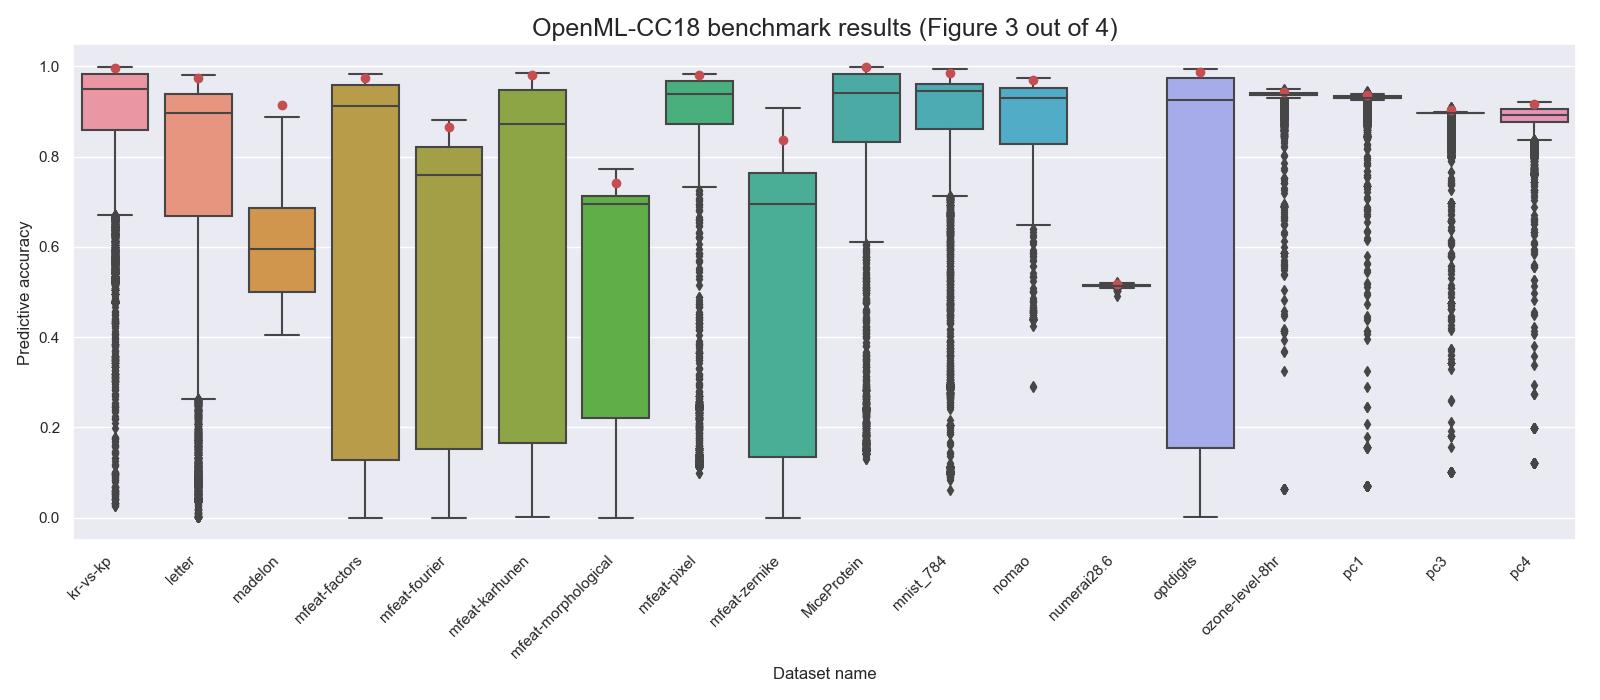
\includegraphics[width=\textwidth]{../img/openml-boxplot2.png}
    \caption[OpenML-CC18 benchmark result comparison (Figure 3 out of 4)]{
	OpenML-CC18 benchmark result comparison (Figure 3 out of 4).    
    Boxplots visualize distributions of predictive accuracies of all
    runs uploaded to OpenML.}
    \label{fig:OpenML:boxplot:2}
\end{sidewaysfigure}

\begin{sidewaysfigure}[ht]
    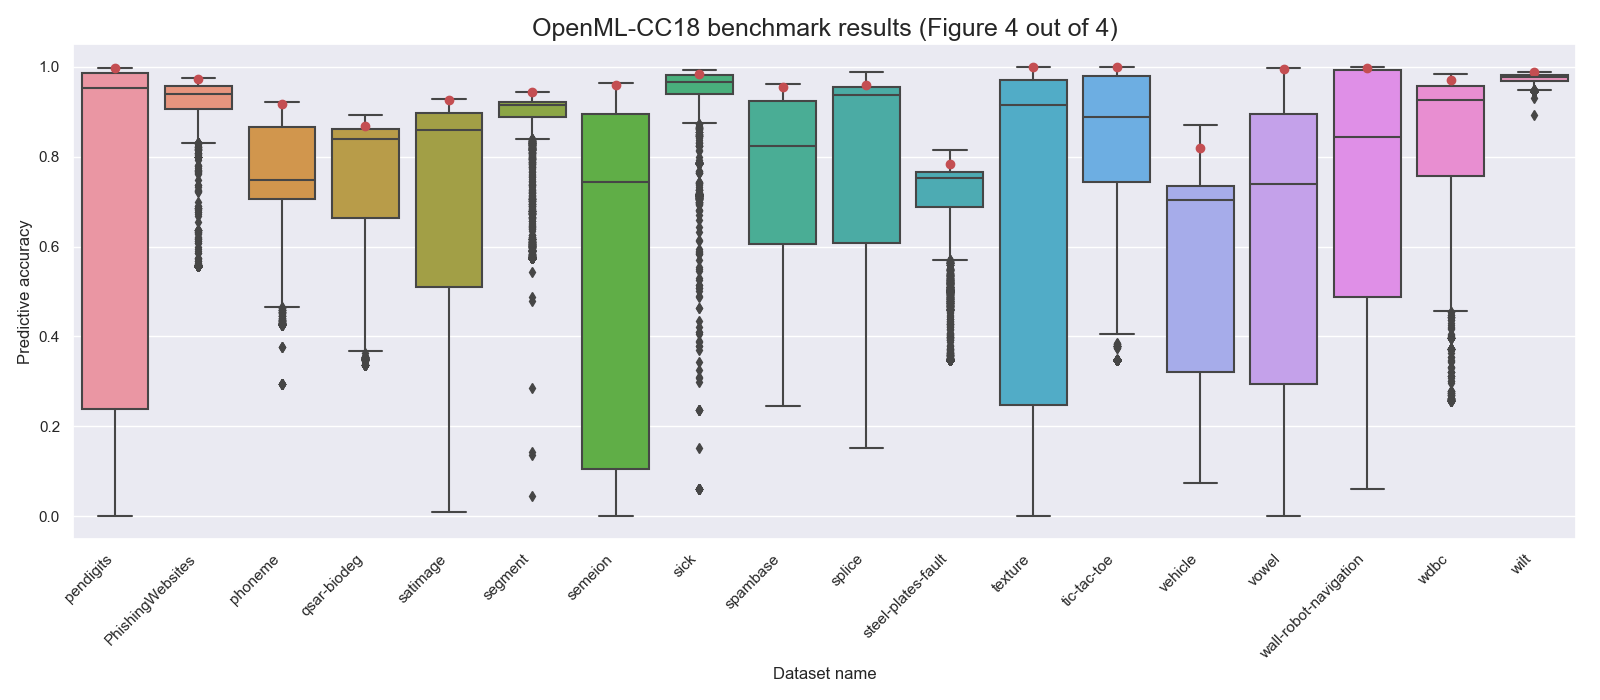
\includegraphics[width=\textwidth]{../img/openml-boxplot3.png}
    \caption[OpenML-CC18 benchmark result comparison (Figure 4 out of 4)]{
    OpenML-CC18 benchmark result comparison (Figure 4 out of 4).
    Boxplots visualize distributions of predictive accuracies of all
    runs uploaded to OpenML.}
    \label{fig:OpenML:boxplot:3}
\end{sidewaysfigure}

% goal - test relationship between per gen and per ind

% Take maximum

% test comparison + describe

% boxplots for comparison (seaborn)
%   - winequality
%   - wilt
%   - magic

% scipt that gets the maximums and makes the plot(s)


\section{Combinations of genetic operators} \label{sec:exp:genop}


\section{OpenML-CC18 benchmarking suite}
% OpenML-CC18
% benchmark description

% TODO pyplot fliers=None vs not